\documentclass[ucs, notheorems]{beamer}

\usetheme[numbers,totalnumbers,compress, nologo]{Statmod}
\usefonttheme[onlymath]{serif}
\setbeamertemplate{navigation symbols}{}

\mode<handout> {
	\usepackage{pgfpages}
	%\setbeameroption{show notes}
	\pgfpagesuselayout{2 on 1}[a4paper, border shrink=5mm]
	\setbeamercolor{note page}{bg=white}
	\setbeamercolor{note title}{bg=gray!10}
	\setbeamercolor{note date}{fg=gray!10}
}

\usepackage[utf8x]{inputenc}
\usepackage[T2A]{fontenc}
\usepackage[russian]{babel}
\usepackage{tikz}
\usepackage{ragged2e}



\newtheorem{theorem}{Теорема}
\newtheorem*{definition}{Определение}
\newtheorem{lemma}{Лемма}
\usepackage{amsmath}
\usepackage{amsthm}
\usepackage{bm}
\usepackage{bbold}
\usepackage{subfigure}

\DeclareMathOperator{\tr}{tr}

\title[Улучшение разделимости для автоматизации SSA]{Улучшение разделимости для автоматизации метода SSA}
\author[Дудник~П. Д.]{ Дудник Павел Дмитриевич, 19Б.04-мм}
\institute[Санкт-Петербургский Государственный Университет]{%
	\small
	Санкт-Петербургский государственный университет\\
	Прикладная математика и информатика\\
	Вычислительная стохастика и статистические модели\\
	\vspace{1.25cm}
	Отчет по производственной практике}
\date{\tiny{Санкт-Петербург\\ 2021г.}}
\begin{document}
	
	\begin{frame}
		\titlepage
		\note{Научный руководитель  к.ф.-м.н., доцент Голяндина Н.\,Э.,\\
			кафедра статистического моделирования}
	\end{frame}
	\begin{frame}{Постановка задачи}
    $F_N = (f_1, \ldots, f_N)$ --- \textbf{временной ряд} длины $N$, $f_i \in \mathbb{R}$ --- наблюдение в момент времени $i$. \\
    \pause
    $F_N = F_{Signal} + F_{Noise}$, --- временной ряд, где $F_{Signal} = F_{Trend} + F_{Periodics}$ - детерминированная составляющая; $F_{Trend}, F_{Periodics}, F_{Noise}$ - временные ряды длины N, компоненты ряда $F$.
    \begin{itemize}
        \item $F_{Trend}$ --- тренд, медленно меняющаяся компонента
        \item $F_{Periodics}$ --- остаток, сумма периодических компонент
        \item $F_{Noise}$ --- шум, случайная составляющая
    \end{itemize}
    \pause
    \textcolor{blue}{Задача}: необходимо придумать и реализовать программу, которая для заданного временного ряда вида $F_N$ автоматически получает его тренд (приближенно). Решение должно использовать алгоритм SSA.
    \note{Пусть имеется временной ряд конечной длины.\\
            Известно, что он имеет следующую модель: ряд состоит из детерминированной составляющей (сигнала) и случайной (шума), сигнал в свою очередь состоит из тренда (медленно меняющейся компоненты) и остатка (суммы периодических компонент).
\\ Нужно создать программу, которая для заданного временного ряда будет автоматически получать его тренд, решение основано на алгоритме SSA.}
\end{frame}


\begin{frame}{"Гусеница" $-$ SSA}
	$F_N=(f_1, \ldots, f_N)$ --- временной ряд, N --- его длина. $1<L<N$ --- длина окна.\\
	\small
	\begin{enumerate}
	    \footnotesize
	    \item \textbf{Вложение}: $K=N-L+1$, ряд переводится в траекторную матрицу $\bm{X}=[X_1:\ldots:X_K]$, где $X_i = (f_i, \ldots, f_{i + L - 1})^{\mathsf{T}}$, $1 \leq i \leq K$.
	    \pause
	    \item \textbf{SVD} траекторной матрицы: $\bm{X} = \sum\limits_{i=1}^d \sqrt{\lambda_i}U_iV_i^{\mathsf{T}} = \sum\limits_{i=1}^d\bm{X}_i$, $1 \leq i \leq d = rank\bm{X}$, $\sqrt{\lambda_i}$ --- сингулярные числа, $\bm{X}_i$ --- траекторная матрица элементарной компоненты (нек. временного ряда).
	    \pause
	    \item \textbf{Группировка}: $\bm{X} =  \sum\limits_{i=1}^r \widetilde{\bm{X}}_i$, где $\widetilde{\bm{X}}_i$ --- траекторная матрица компоненты, состоящей из одной или нескольких элементарных компонент, r --- число компонент.
	    \pause
	    \item \textbf{Диагонализация}: каждая тр. матрица компоненты переводится во временной ряд.
	\end{enumerate}
	Результат работы "Гусеницы" $-$ SSA --- разложение временного ряда в сумму компонент.

	\note{	\footnotesize Рассмотрим сам алгоритм SSA: пусть у нас есть временной ряд с известной моделью, есть параметр $L$ --- длина окна, сначала выполняется вложение (из ряда извлекаются вектора, полученные последовательным сдвигом окна), помещаем их в столбцы, полученная матрица называется траекторной.
\\Строится сингулярное разложение, получаем представление траекторной матрицы в виде суммы траекторных матриц элементарных компонент (элементарной компонентой будем называть ряд, который соответствует одному слагаемому в сумме)
\\ Далее слагаемые группируются некоторым образом (обычно, на основе анализа, в том числе визуального, вручную) и суммируются внутри группы, получаем представление в виде суммы траекторных матриц компонент.
\\ Далее каждое слагаемое переводится в ряд c помощью диагонального усреднения.
Таким образом результат работы - разложение временного ряда в сумму компонент.}
\end{frame}

\begin{frame}{Пример применения метода SSA}
\small
    Ряд: сумма тренда $0.001n^2 - 0.5n + 3$ и гармоники $2 \cos(\frac{2 \pi n} {3})$.
    \pause
    \begin{figure}
  \begin{minipage}[c]{0.5\textwidth}
    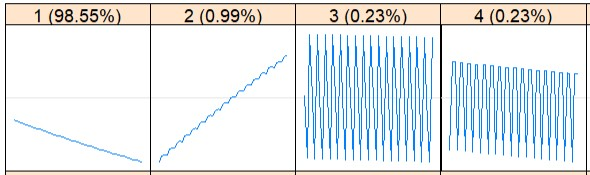
\includegraphics[scale = 0.4]{ssa_example1.jpg}
  \end{minipage}\hfill
  \begin{minipage}[l]{0.5\textwidth}
    \caption{
       \footnotesize График $U_i$ (график на основе SVD)
    } \label{fig:03-03}
  \end{minipage}
\end{figure}
    \pause
    \begin{figure}
  \begin{minipage}[c]{0.5\textwidth}
    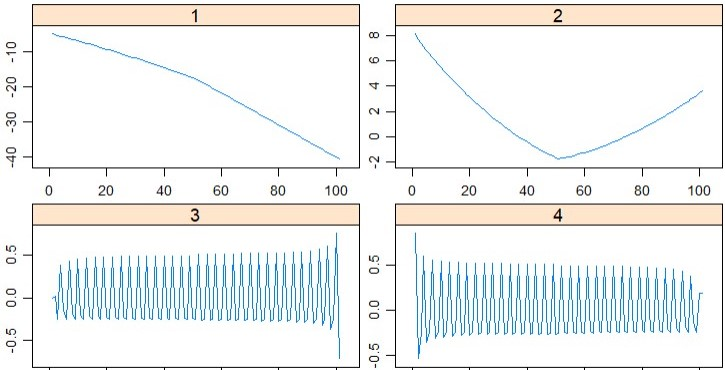
\includegraphics[scale = 0.3]{ssa_example2.jpg}
  \end{minipage}\hfill
  \begin{minipage}[l]{0.5\textwidth}
    \caption{
       Элементарные компоненты ряда
    } \label{fig:03-03}
  \end{minipage}
\end{figure}

\begin{figure}
  \begin{minipage}[c]{0.5\textwidth}
    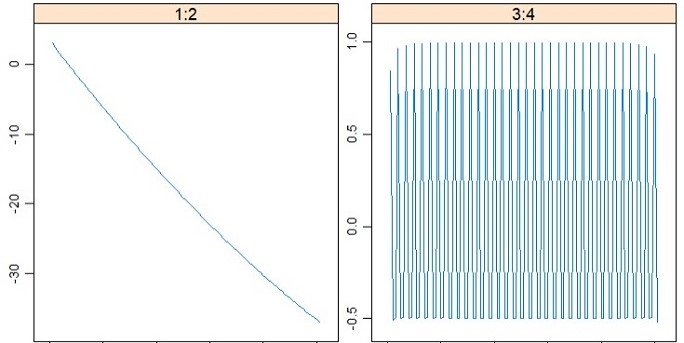
\includegraphics[scale = 0.3]{ssa_example3.jpg}
  \end{minipage}\hfill
  \begin{minipage}[l]{0.5\textwidth}
    \caption{
       Восстановленные тренд и гармоника
    } \label{fig:03-03}
  \end{minipage}
\end{figure}
    
    \note{Рассмотрим временной ряд, состоящий из тренда и гармоники.\\
    Для произведения шага группировки исследуются так называемые факторные вектора, которые участвуют в сингулярном разложении. Взглянем на них: первые два вектора, которые относятся к первым двум элементарным компонентам, похожи на медленно меняющиеся ряды, два другие --- на гармоники. С помощью таких рассуждений мы отнесем первые две элементарные компоненты к тренду, остальные --- к периодикам. \\
    Рассмотрим графики элементарных компонент этого ряда. Действительно, графики показывают, что по виду факторных векторов можно сказать, чем является элементарная компонента.\\
    Таким образом, отнесем первые две элементарные компоненты к тренду, остальные --- к периодикам и посмотрим, восстановился ли тренд и периодики.\\
    Действительно, мы получили заданные тренд и гармонику. Таким образом, результат работы алгоритма SSA --- это разложение ряда в сумму компонент.
    }
\end{frame}


\begin{frame}{Автоматическое извлечение тренда}
    \textcolor{blue}{Проблема}: группировка производится на основе визуального анализа.\\
    \pause
    Можно использовать разложение Фурье:
    \small
    \begin{equation*}
        f_n = c_0 + \sum\limits_{k = 1}^{\lfloor \frac{N - 1}{2}\rfloor} \sqrt{c_k^2 + s_k^2}cos(\frac{2\pi nk}{N} + \phi_k) + c_{\frac{N}{2}}(-1)^k
    \end{equation*}\\
    Тренд --- составляющая, в которую большой вклад вносят только низкие частоты в разложении Фурье.\\
    \pause
    \small
    \begin{equation*}
                \Pi^f_N (\frac{k}{N}) = \frac{N}{2}
        \begin{cases}
        2c_0^2 & ,k = 0\\
        c_k^2+s_k^2 & ,0 < k < N/2\\
        2c^2_{N/2} & ,k = N/2
        \end{cases}
    \end{equation*}
    Относим элементарные компоненты, у которых $\sum\limits_{0 \leq \frac{k}{N} < \omega_0}\Pi_N^f(\frac{k}{N}) > T_0$, к тренду. Назовем $T_0$ вкладом низких частот.
    \note{Как было сказано, группировка элементарных компонент выполняется вручную. Возникает необходимость проводить группировку автоматически. Для извлечения тренда, например, можно использовать разложение Фурье. \\
    Определим тренд как составляющую, у которой большой вклад низких частот. С помощью следующей функции, которая называется периодограмма ряда, можно формализовать понятие вклада. Назовем вкладом сумму периодограмм по частотам, которые меньше некоторой небольшой фиксированной частоты. \\
    Тогда, если вклад больше фиксированного порога, будем относить элементарную компоненту к тренду.}
\end{frame}

\begin{frame}{Пример автоматического выделения тренда}
    Ряд: сумма тренда $0.001n^2 - 0.5n + 3$ и гармоники $2 \cos(\frac{2 \pi n} {3})$.\\
    \pause
    Выберем $\omega_0 = \frac{1}{24}$, $T_0$ = 0.8.\\
    \pause
    \begin{table}[h]
        \caption{\footnotesize Вклад низких частот в эл. компоненты}
        \begin{center}
        \tabcolsep=0.11cm
        \begin{tabular}{|l | c| c| c| c| c| c|}
        \hline
         & 1 & 2 & 3 & 4\\
         \hline
         Вклад & 0.97 & 0.97 & 0.001 & 0.001\\
        \hline
        \end{tabular}
        \end{center}
    \end{table}
    \pause
    Относим эл. компоненты 1 и 2 к тренду.
    
    \note{Снова обратимся к примеру. Выберем ограничивающую частоту $\frac{1}{24}$ и порог 0.8.\\
    Взглянем на вклады низких частот в элементарные компоненты. Видно, что значение вклада больше для первой и второй элементарной компоненты. Следовательно, их необходимо отнести к тренду. \\
    Как было показано ранее, первые две элементарные компоненты действительно относятся к тренду.}
\end{frame}

\begin{frame}{Разделимость компонент}
    \begin{itemize}
        \item \textcolor{blue}{Проблема}: если не существует представления тренда в виде суммы некоторых эл. компонент в SSA, то автоматическое выделение тренда невозможно.
        \pause
        \item Тренд и остаток \textbf{разделимы}, понятие разделимости включает в себя биортогональность траекторных матриц компонент.
    \end{itemize}
    \pause
    \vspace{5pt}
    \begin{center}
    \begin{tikzpicture}[>=latex]
    \node[draw,rectangle,inner sep=5pt] (yes) at (2,0.5)
    {\small Автоматическая идентификация};
    \node[draw,rectangle,inner sep=5pt] (no) at (2,1.8)
    {\small \ \ \ \ \ Получение разделимости \ \ \ \ \ };
    \draw[->] (no) -> (yes);
    \end{tikzpicture}
    \end{center}

    \begin{itemize}
        \pause
        \item Идея: можно \textbf{ослабить} условие ортогональности.
    \end{itemize}
    \note{
    Однако существует проблема недостатка разделимости: мы можем произвести автоматическую идентификацию тренда только в том случае, если траекторной матрице тренда и остатка соответствуют некоторые матрицы элементарных компонент. \\
Другими словами, нам нужно, чтобы тренд и остаток были разделимы, понятие разделимости рядов включает в себя биортогональность траекторных матриц.
\\
Для решения проблемы необходимо получить разделимость тренда и остатка.
Ослабим условие ортогональности.
    }
\end{frame}

\begin{frame}{Пример с отсутствием разделимости}
    Ряд: сумма тренда $0.001n^2 - 0.5n + 3$ и гармоники $2 \cos(\frac{2 \pi n} {3})$.\\
    \pause
    \begin{figure}
      \begin{minipage}[c]{0.5\textwidth}
        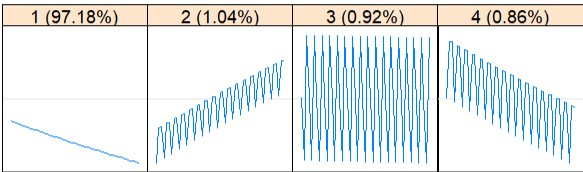
\includegraphics[scale = 0.4]{ssa_example4.jpg}
      \end{minipage}\hfill
      \begin{minipage}[l]{0.5\textwidth}
        \caption{
           \footnotesize График $U_i$ (график на основе SVD)
        } \label{fig:03-03}
      \end{minipage}
    \end{figure}
    Чему равны вклады низких частот?\\
    \pause
    \begin{table}[h]
            \caption{\footnotesize Вклад низких частот в эл. компоненты}
            \footnotesize
            %\tabcolsep = 0.11cm
            \begin{tabular}{|l | c| c| c| c|}
            \hline
             & 1 & 2 & 3 & 4\\
             \hline
             Вклад & 0.97 & 0.82 & 0 & 0.45 \\
            \hline
            \end{tabular}

        \end{table}

    \begin{figure}
      \begin{minipage}[l]{0.5\textwidth}
        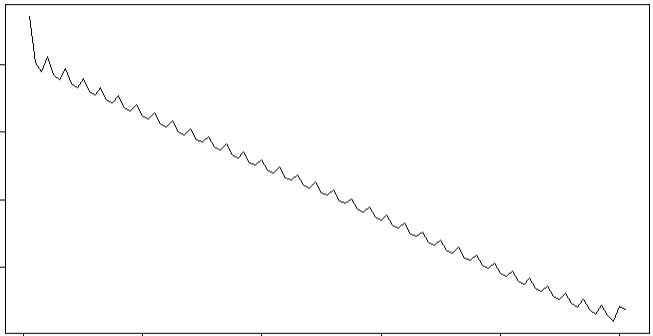
\includegraphics[scale = 0.33]{ssa_example5.jpg}
      \end{minipage}\hfill
      \begin{minipage}[l]{0.5\textwidth}
        \caption{
           \footnotesize Восстановленный тренд
        } \label{fig:03-03}
      \end{minipage}
    \end{figure}

    \pause
    \note{Рассмотрим тот же временной ряд, при изменив амплитуду гармоники, т.е. коэффициент при функции косинус. Попробуем в этом примере определить, куда отнести компоненты, посмотрим на факторные вектора.\\
    Видно, что некоторые векторы похожи и на тренд, и на гармонику.\\
    Попробуем воспользоваться автоматическим выделением тренда. Посмотрим на вклады низких частот.\\
    У первых двух элементарных компонент вклад больше порога, объединим их в одну компоненту и восстановим.\\
    Как можно увидеть, тренд выделился неверно, в этом и состоит проблема отсутствия разделимости. Обратимся в методам, позволяющим решить эту проблему.}
    
\end{frame}

\begin{frame}{Oblique SSA}
    Идея \textbf{Oblique SSA}: переопределение скалярного произведения.
    \begin{center}
        $\langle X_1,X_2\rangle_{\bm{A}} = (\mathbf{A}X_1,X_2)$
    \end{center}
    \pause
    Ряд конечного ранга, управляемый ЛРФ: $s_{r+i} = a_1s_{r+i - 1} + a_2s_{r+i - 2} + . . . + a_rs_i
, \forall i \in 1, . . . , N - r$
    Характеристический полином ЛРФ:
    \begin{equation*}
        \chi_{\mathbf{a}} (\mu ) = \mu^r - \sum^r_{k=1} a_k\mu^{r - k}
    \end{equation*}
    \pause
    
    Для любого ряда конечного ранга с различными корнями х.п. $\mathbb{Y} = \mathbb{Y}_1 + \mathbb{Y}_2$ можно переопределить $( - , - )$ так, чтобы компоненты $\mathbb{Y}_1, \mathbb{Y}_2$ стали разделимы (в новых условиях ортогональности).
    \note{Рассмотрим модификацию SSA, косоугольный SSA. В нем сингулярное разложение строится с переопределенным скалярным произведением, тем самым ослабляется условие ортогональности, затем производится группировка, так же, как и в базовом алгоритме.\\
    Рассмотрим при этом понятия рядов конечного ранга, управляемых линейной рекуррентной формулой. Для таких рядов всегда можно переопределить скалярное произведение так, чтобы их разделить.

    Однако, существует следующая проблема: если мы не знаем пространства строк и столбцов траекторных матриц компонент, то мы не можем переопределить скалярное произведение, чтобы получить разделимость.
    }
\end{frame}

\begin{frame}{IOSSA, EOSSA}
    \small
    \textbf{IOSSA} (Iterative Oblique SSA): Итеративная версия Nested OSSA.

    \begin{itemize}
    \small
        \item \textbf{Начальная группировка}: группировка слагаемых сигнала в SVD (набор из наборов индексов).
        \pause
        \item IOSSA требуется некоторое количество итераций до сходимости.
    \end{itemize}
    \begin{figure}[h]
    \center{\includegraphics[scale=0.7]{iossa 2.jpg}}
    \caption{\footnotesize Пример вызова метода IOSSA, начальная группировка --- 2 компоненты}
    \label{fig:image}
    \end{figure}
    \pause
    \textbf{EOSSA} (ESPRIT-motivated Oblique SSA): метод разделения сигнала, использующий собственные подпространства сдвиговых матриц.
    \pause
    Методы применимы для разделения компонент ряда с непересекающимися множествами корней их х.п. $\chi_{\mathbf{a}} (\mu )$

    \note{Используем итеративную версию этого алгоритма: IOSSA. Этот метод итеративно переопределяет скалярное произведение. У этого алгоритма есть параметр начальная группировка: мы задаём, какие элементарные компоненты будут на начальных итерациях отнесены к сигналу, а также как их следует объединить в компоненты на начальных итерациях. При этом группировка может меняться на каждой итерации.\\
Также этому алгоритму необходимо некоторое количество итераций, чтобы алгоритм сошёлся.\\
Существует также еще один метод, позволяющий получить разделимость компонент --- EOSSA: этот алгоритм разделяет сигнал при помощи собственных подпространств сдвиговых матриц. Более подробно этот алгоритм будет рассмотрен во второй части работы. Стоит отметить, что применимость этого метода ограниченна: мы можем его применять только в том случае, если корни характеристического полинома (так называемые сигнальные корни) различны.}
\end{frame}

\begin{frame}{Пример получения разделимости}
    Ряд: сумма тренда $0.001n^2 - 0.5n + 3$ и гармоники $2 \cos(\frac{2 \pi n} {3})$.\\
    \note{Обратимся к примеру, в котором не было разделимости тренда и гармоники.\\
    Используем алгоритм IOSSA. Поместим в качестве начальной группировки в первую группу первую и вторую элементарные компоненты, во вторую группу соответственно третью и четвертую.
    
    }    
\end{frame}

\begin{frame}{Автоматизация выделения тренда с помощью IOSSA}
    \textbf{Ручная начальная группировка}
        \footnotesize
        \begin{itemize}
            \item IOSSA, начальная группировка --- визуальный анализ.
            \item Автоматическая идентификация:  тренд --- одна компонента.
        \end{itemize}
        \pause
        \normalsize
    \textbf{Автоматическая начальная группировка} (решение)
        \footnotesize
        \begin{itemize}
            \item IOSSA, начальная группировка: одна группа --- элементарные компоненты с большим вкладом низких частот, другая --- остальные.
            \item Автоматическая идентификация: тренд --- одна компонента.
        \end{itemize}
        \pause
        \normalsize
    \textbf{Без начальной группировки} (еще одно решение)
        \footnotesize
        \begin{itemize}
            \item IOSSA, начальная группировка:  k групп по одной элементарной компоненте, где k - количество элементарных компонент в сигнале.
            \item Автоматическая идентификация: тренду соответствует одна или несколько элементарных компонент.
        \end{itemize}
        \note{Рассмотрим способы получения тренда, можно использовать IOSSA, затем сделать автоматическое выделение тренда, группировка не автоматическая, получаем тренд одной компонентой.\\
        Отметим, что начальная группировка может привести к неправильному разделению, если размеры групп индексов в ней не совпадают с рангами нужных компонент (в нашем случае, тренда и компоненты с периодиками).
\\ Далее следующее решение: в начальную группировку IOSSA передаём элементарные компоненты сигнала, у которых большой вклад низких частот, после применения iossa предполагаемый тренд - одна компонента.
\\ Ещё одно решение: в начальной группировке IOSSA группа - это элементарная компонента сигнала, после применения IOSSA тренду соответствует несколько компонент. Далее применяется идентификация тренда через низкие частоты.}
\end{frame}

\begin{frame}{Автоматизация выделения тренда (SSA, EOSSA)}
    \textbf{Базовый алгоритм}
        \begin{itemize}
        \small
            \item Применяется базовый алгоритм SSA.
            \item Автоматическая идентификация:  тренд --- одна компонента.
            \item Этот метод не решает проблему недостатка разделимости
        \end{itemize}
        \pause
        \normalsize
    \textbf{Алгоритм, использующий EOSSA} (решение)

        \begin{itemize}
        \small
            \item Параметр: индексы, относящиеся к сигналу.
            \item Автоматическая идентификация: тренд --- одна компонента.
            \pause
            \item Это решение подходит только для рядов конечного ранга с различными корнями $\chi_{\mathbf{a}} (\mu )$.
        \end{itemize}
        \begin{figure}[h]
    \center{\includegraphics[scale=0.7]{eossa 2.jpg}}
    \caption{\footnotesize Пример вызова метода EOSSA, 2 компоненты}
    \label{fig:image}
    \end{figure}
        
\note{Рассмотрим также метод, который использует только базовый алгоритм. В этом методе на этапе группировки восстанавливаются все элементарные компоненты и применяется автоматическое извлечение тренда. Как уже сказано ранее, этот метод при недостатке разделимости дает неверную оценку компонент.

Также рассмотрим решение, которое использует EOSSA. Чтобы получить нужное разложение, достаточно указать компоненты, относящиеся к сигналу, и нужное количество компонент в разложении. Применимость такого решения ограниченна моделью ряда с различными сигнальными корнями.}
\end{frame}

\begin{frame}{Численные эксперименты}
\small
    Было проведено два эксперимента для сравнения методов, использовался временной ряд длины $N = 101$: сумма тренда, одной или двух гармоник и белого гауссовского шума. Длина окна $L = 48$.
    \pause
    Эксперимент 1
    \begin{itemize}
        \item Тренд $-0.2 e^{0.03n}$
        \item Гармоника (остаток) $2.65 \mathsf{cos}(\frac{2\pi n}{3})$
        \item Шум: ${N}(0, 0.04)$
    \end{itemize}
\pause
\begin{table}[h]
\tiny
\caption{\footnotesize Сравнение решений}
\begin{center}
\tabcolsep=0.11cm
\begin{tabular}{|l | c| c| c| c| c| c|}
\hline
 & \multicolumn{2}{c|}{Выделение тренда} & \multicolumn{2}{c|}{Выделение остатка} & \multicolumn{2}{c|}{Количество итераций} \\
 \hline
 & MSE, mean & MSE, med & MSE, mean & MSE, med & mean & med  \\
\hline
no grouping & 0.0016 &  0.0013 & 0.0029 &  0.0026 & 7 & 3 \\
manual grouping &  0.0014 & 0.0011 & 0.0027 & 0.0024 & 3 & 3 \\
auto grouping &  9e-04 & 6e-04 & 0.0022 & 0.002 & 3 & 3 \\
\hline
eossa & 9e-04 & 6e-04 & 0.0022 & 0.002 & \multicolumn{2}{c|}{-} \\
basic\_ssa &  0.1756 & 0.0917 & 0.1822 & 0.0852  & \multicolumn{2}{c|}{-} \\
\hline
\end{tabular}
\end{center}
\end{table}
\note{Перейдем к экспериментам. Во всех экспериментах использовался ряд с отсутствием сильной разделимости тренда и периодик, чтобы наглядно продемонстрировать проблему отсутствия разделимости. Тренд в этом примере простой, он состоит из одной элементарной компоненты. Использовалась одна гармоника и небольшой гауссовский белый шум.\\
Согласно результатам, полученным в результате эксперимента (результаты отра
жены в таблице), решению, использующему IOSSA без начальной группировки,
потребовалось чуть большее количество итераций, по сравнению остальными решения
ми, использующими IOSSA. При этом можно увидеть, что у всех методов, основанных
на Oblique SSA (первые 4 метода), ошибка выделения тренда и остатка примерно оди
наковая. Если посмотреть на результат метода, основанного на базовом алгоритме, то
можно увидеть, что ошибка выделения тренда и остатка больше, чем у других методов,
на два порядка.}

\end{frame}

\begin{frame}{Численные эксперименты}
\small

    Эксперимент 2
    \begin{itemize}
        \item Тренд $2e^{0.03n} - 0.1n - 20$
        \item Гармоники (остаток) $5.2\mathsf{cos}(\frac{2\pi n}{6} + \frac{\pi}{4})$, $5.2\mathsf{cos}(\frac{2 \pi n} {3})$
        \item Шум: ${N}(0, 0.04)$
    \end{itemize}
\pause
\begin{table}[H]
\tiny
\caption{Сравнение решений}
\begin{center}
\begin{tabular}{|l | c| c| c| c| c| c|}

\hline
& \multicolumn{2}{c|}{Выделение тренда} & \multicolumn{2}{c|}{Выделение остатка} & \multicolumn{2}{c|}{Количество итераций} \\
 \hline
 & MSE, mean & MSE, med & MSE, mean & MSE, med & mean & med  \\
\hline
no grouping &  0.0031 & 0.0029 & 0.0054 & 0.0049 & 477 & 372 \\
manual grouping & 0.0022 & 0.0019 & 0.0046 & 0.0044 & 4 & 4 \\
auto grouping &  0.3337 & 0.0017 & 0.3268 & 0.0044 & 5 & 4 \\
\hline
eossa &  0.0019 & 0.0016 & 0.0044 & 0.0041 & \multicolumn{2}{c|}{-} \\
basic\_ssa &  5.9826 & 2.9367 & 5.9596 & 2.9348 & \multicolumn{2}{c|}{-} \\
\hline
\end{tabular}
\end{center}
\end{table}
    \note{\footnotesize Во втором эксперименте использовался более сложный тренд, также использовались две гармоники. \\
    Согласно результатам, полученным в результате эксперимента, решению, использующему IOSSA без начальной группировки,
потребовалось большое количество итераций. При этом можно увидеть, что медианное количество итераций значительно меньше среднего, что говорит о некотором количестве случаев, когда сходимость затруднялась.\\
Средняя ошибка и медианная ошибки выделения тренда и остатка для метода, использующего IOSSA с автоматической начальной группировкой, говорит о некотором количестве неудачных начальных группировок.\\
Можно отметить, что решение, использующее IOSSA без начальной группировки,и решение, использующее EOSSA, показали устойчивый результат: средние ошибки выделения примерно равны медианным.
Метод, использующий базовый метод SSA, показал большую ошибку.}
\end{frame}

\begin{frame}{Выводы из экспериментов}
    \begin{itemize}
        \item Базовый метод не подходит для рядов с недостатком разделимости.
        \pause
        \item Решению, использующему IOSSA без начальной группировки, потребовалось большое количество итераций для сходимости.
        \pause
        \item Решение, использующеее IOSSA с автоматической начальной группировкой, может получить неточное разделение.
    \end{itemize}
    \note{\small Подведем итог. \\
    Метод, использующий базовый алгоритм SSA, показал в обоих экспериментах большую ошибку. Это неслучайно: в экспериментах не было сильной разделимости тренда и периодик, поэтому, разложение получалось неверным.\\
В эксперименте со сложным трендом решению, использующему
IOSSA без начальной группировки, потребовалось большое количество итераций для сходимости. Этот метод можно использовать для решения задачи в том случае, если устраивает большое время работы, и при этом нужна устойчивость и точность. Если же необходимо небольшое время работы и при этом точность не так важна, то можно использовать решение с автоматической начальной группировкой.\\
Также в качестве решения, автоматически выделяющего тренд, можно взять метод, использующий EOSSA. Однако существуют ограничения для применимости этого
метода (несовпадение сигнальных корней). Это послужило мотивацией к модификации метода, что было проделано во второй части работы.
}
\end{frame}
	
\begin{frame}{Обобщение метода EOSSA на случай кратных корней}
    \begin{theorem}
    Ряд $\mathbb{S}$ конечного ранга $r$ с различными $\{ \mu_i\}$. Пусть имеется минимальное разложение $\mathbf{S} = \mathbf{PQ}^{\mathrm{T}}$
    Тогда:
    \begin{itemize}
        \item Существует $\mathbf{M} \in \mathbb{C}^{r \times r}$: $\overline{\mathbf{P}} = \underline{\mathbf{P}}\mathbf{M}$.
        \item  Собственные числа матрицы $\mathbf{M}$ совпадают с корнями х.п. $\mu_k$.
        \item Пусть $\mathbf{M} = \mathbf{T}\mathsf{diag}(\mu_1,\dots,\mu_r)\mathbf{T}^{-1}, \mathbf{T} \in \mathbb{C}^{r \times r}$ - спектральное разложение матрицы $\mathbf{M}$.Тогда $\mathbf{S} = \mathbf{\Pi\Psi}^{\mathrm{T}}$, где матрицы $\mathbf{\Pi} = \mathbf{PT}$ и $\mathbf{\Psi} = \mathbf{Q}(\mathbf{T}^{-1})^{\mathrm{T}}$ имеют Вандермондовскую структуру.
    \end{itemize}
    \end{theorem}
    \note{Для задачи, поставленной в начале, можно использовать алгоритм EOSSA. Однако если рассматривать тренд с кратными сигнальными корнями, то
EOSSA уже нельзя будет применить. Следовательно, существует необходимость в обобщении EOSSA на случай кратных сигнальных корней. \\
Рассмотрим теорему, которая показывает идею EOSSA. Метод получает так называемую сдвиговую матрицу $\mathbf{M}$, ее собственные числа совпадают с сигнальными корнями. Для построения нужного нам разложения траекторной матрицы используются собственные подпространства $\mathbf{M}$, базисные вектора этих пространств получим с помощью спектрального разложения. \\}
\end{frame}

\begin{frame}{Обобщение метода EOSSA на случай кратных корней}
    \begin{theorem}
    Ряд $\mathbb{S}$ конечного ранга $r$. Пусть имеется сингулярное  разложение $\mathbf{S} = \mathbf{P\Sigma Q}^{\mathrm{T}}$
    Тогда:
    \begin{itemize}
        \item Существует $\mathbf{M} \in \mathbb{C}^{r \times r}$: $\overline{\mathbf{P}} = \underline{\mathbf{P}}\mathbf{M}$.
        \item  Собственные числа матрицы $\mathbf{M}$ совпадают с корнями х.п. $\mu_k$, учитывая кратность.
        \item Пусть $\mathbf{M} = \mathbf{TJ}\mathbf{T}^{-1}, \mathbf{T} \in \mathbb{C}^{r \times r}$ - каноническое жорданово представление $\mathbf{M}$.Тогда $\mathbf{S} = \mathbf{\Pi H\Psi}^{\mathrm{T}}$, где матрицы $\mathbf{\Pi} = \mathbf{PT}$ и $\mathbf{\Psi}$ имеют структуру Паскаля-Вандермонда.
    \end{itemize}
    \end{theorem}
    \pause
    \textbf{Результат}: обобщение метода сводится к оценке собственных подпространств матрицы $\mathbf{M}$.\\
    \textbf{Проблема}: нет устойчивых методов получения базиса.
    \note{Так как сигнальные корни их кратности совпадают с собственными числами матрицы сдвига и их кратностями, то можно использовать ту же идею, что используется при несовпадающих корнях --- нужно оценить собственные подпространства матрицы сдвига. \\
    Воспользуемся следующей теоремой, которая несколько отличается от предыдущей. В рассматриваемом случае спектральное разложение поменялось на каноническое жорданово, и если в предыдущем случае можно было легко получить матрицу с базисными векторами, то получить каноническое жорданово представление устойчиво невозможно.\\
    Можно решить проблему оценки собственных подпространств отдельно, не строя разложение. Эту проблему я планирую рассмотреть в будущем, в следующей курсовой работе.}
\end{frame}


	
\end{document}